\documentclass{beamer}

\pdfmapfile{+sansmathaccent.map}


\mode<presentation>
{
  \usetheme{Warsaw} % or try Darmstadt, Madrid, Warsaw, Rochester, CambridgeUS, ...
  \usecolortheme{seahorse} % or try seahorse, beaver, crane, wolverine, ...
  \usefonttheme{serif}  % or try serif, structurebold, ...
  \setbeamertemplate{navigation symbols}{}
  \setbeamertemplate{caption}[numbered]
} 


%%%%%%%%%%%%%%%%%%%%%%%%%%%%
% itemize settings

\definecolor{mypink}{RGB}{255, 30, 80}
\definecolor{mydarkblue}{RGB}{60, 160, 255}
\definecolor{myblue}{RGB}{240, 240, 255}
\definecolor{mygreen}{RGB}{0, 200, 0}
\definecolor{mygreen2}{RGB}{245, 255, 230}
\definecolor{mygray}{gray}{0.8}

\setbeamertemplate{itemize items}[default]

\setbeamertemplate{itemize item}{\color{mygreen}$\blacksquare$}
\setbeamertemplate{itemize subitem}{\color{mydarkblue}$\blacktriangleright$}
\setbeamertemplate{itemize subsubitem}{\color{mygray}$\blacksquare$}



\setbeamercolor{palette quaternary}{fg=white,bg=mydarkblue}
\setbeamercolor{titlelike}{parent=palette quaternary}

\setbeamercolor{palette quaternary2}{fg=black,bg=myblue}
\setbeamercolor{frametitle}{parent=palette quaternary2}



\setbeamerfont{frametitle}{size=\Large,series=\scshape}
\setbeamerfont{framesubtitle}{size=\normalsize,series=\upshape}





%%%%%%%%%%%%%%%%%%%%%%%%%%%%
% block settings

\setbeamercolor{block title}{bg=red!30,fg=black}

\setbeamercolor*{block title example}{bg=mygreen!40!white,fg=black}

\setbeamercolor*{block body example}{fg= black,
bg= mygreen2}


%%%%%%%%%%%%%%%%%%%%%%%%%%%%
% URL settings
\hypersetup{
    colorlinks=false,
    linkcolor=blue,
    filecolor=blue,      
    urlcolor=blue,
}

%%%%%%%%%%%%%%%%%%%%%%%%%%

\renewcommand{\familydefault}{\rmdefault}

\usepackage{amsmath}
\usepackage{mathtools}


\usepackage{subcaption}

\newcommand{\bo}[1] {\mathbf{#1}}
\newcommand{\R} {\mathbb{R}}
\DeclareMathOperator*{\argmin}{arg\,min}


%%%%%%%%%%%%%%%%%%%%%%%%%%%%
% code settings

\usepackage{listings}
\usepackage{color}
% \definecolor{mygreen}{rgb}{0,0.6,0}
% \definecolor{mygray}{rgb}{0.5,0.5,0.5}
\definecolor{mymauve}{rgb}{0.58,0,0.82}
\lstset{ 
  backgroundcolor=\color{white},   % choose the background color; you must add \usepackage{color} or \usepackage{xcolor}; should come as last argument
  basicstyle=\footnotesize,        % the size of the fonts that are used for the code
  breakatwhitespace=false,         % sets if automatic breaks should only happen at whitespace
  breaklines=true,                 % sets automatic line breaking
  captionpos=b,                    % sets the caption-position to bottom
  commentstyle=\color{mygreen},    % comment style
  deletekeywords={...},            % if you want to delete keywords from the given language
  escapeinside={\%*}{*)},          % if you want to add LaTeX within your code
  extendedchars=true,              % lets you use non-ASCII characters; for 8-bits encodings only, does not work with UTF-8
  firstnumber=0000,                % start line enumeration with line 0000
  frame=single,	                   % adds a frame around the code
  keepspaces=true,                 % keeps spaces in text, useful for keeping indentation of code (possibly needs columns=flexible)
  keywordstyle=\color{blue},       % keyword style
  language=Octave,                 % the language of the code
  morekeywords={*,...},            % if you want to add more keywords to the set
  numbers=left,                    % where to put the line-numbers; possible values are (none, left, right)
  numbersep=5pt,                   % how far the line-numbers are from the code
  numberstyle=\tiny\color{mygray}, % the style that is used for the line-numbers
  rulecolor=\color{black},         % if not set, the frame-color may be changed on line-breaks within not-black text (e.g. comments (green here))
  showspaces=false,                % show spaces everywhere adding particular underscores; it overrides 'showstringspaces'
  showstringspaces=false,          % underline spaces within strings only
  showtabs=false,                  % show tabs within strings adding particular underscores
  stepnumber=2,                    % the step between two line-numbers. If it's 1, each line will be numbered
  stringstyle=\color{mymauve},     % string literal style
  tabsize=2,	                   % sets default tabsize to 2 spaces
  title=\lstname                   % show the filename of files included with \lstinputlisting; also try caption instead of title
}

%%%%%%%%%%%%%%%%%%%%%%%%%%%%
% tikz settings

\usepackage{tikz}
\tikzset{every picture/.style={line width=0.75pt}}

%%%%%%%%%%%%%%%%%%%%%%%%%%%%

\usepackage{qrcode}



\title{Introduction, linear system representations}
\subtitle{Control Theory, Lecture 1}
\author{by Sergei Savin}
\centering
\date{Spring 2022}



\begin{document}
\maketitle


\begin{frame}{Content}

\begin{itemize}
\item Motivation
\item Ordinary differential equations
    \begin{itemize}
    \item 1st order
    \item n-th order
    \end{itemize}
\item Linear differential equations
    \begin{itemize}
    \item 1st order
    \item n-th order
    \item ...are what we will study
    \end{itemize}
\item Changing n-th order ODE to a State-Space form
\item Read more
\end{itemize}

\end{frame}



\begin{frame}{What is control?}
% \framesubtitle{O}
\begin{flushleft}

The first obvious question is, what is control theory? The easiest strategy to answer this question is to bring examples of systems that you can \emph{learn how to control}:

\begin{figure}
\minipage{0.45\textwidth}
  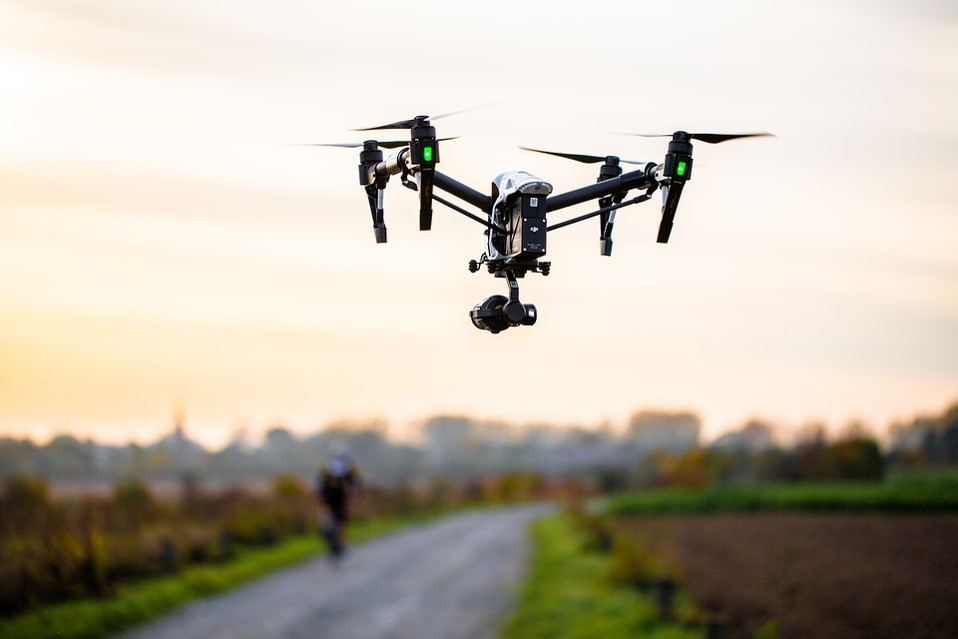
\includegraphics[width=\linewidth]{Picture1.jpg}
  \caption{Drone}
\endminipage\hfill
\minipage{0.45\textwidth}
  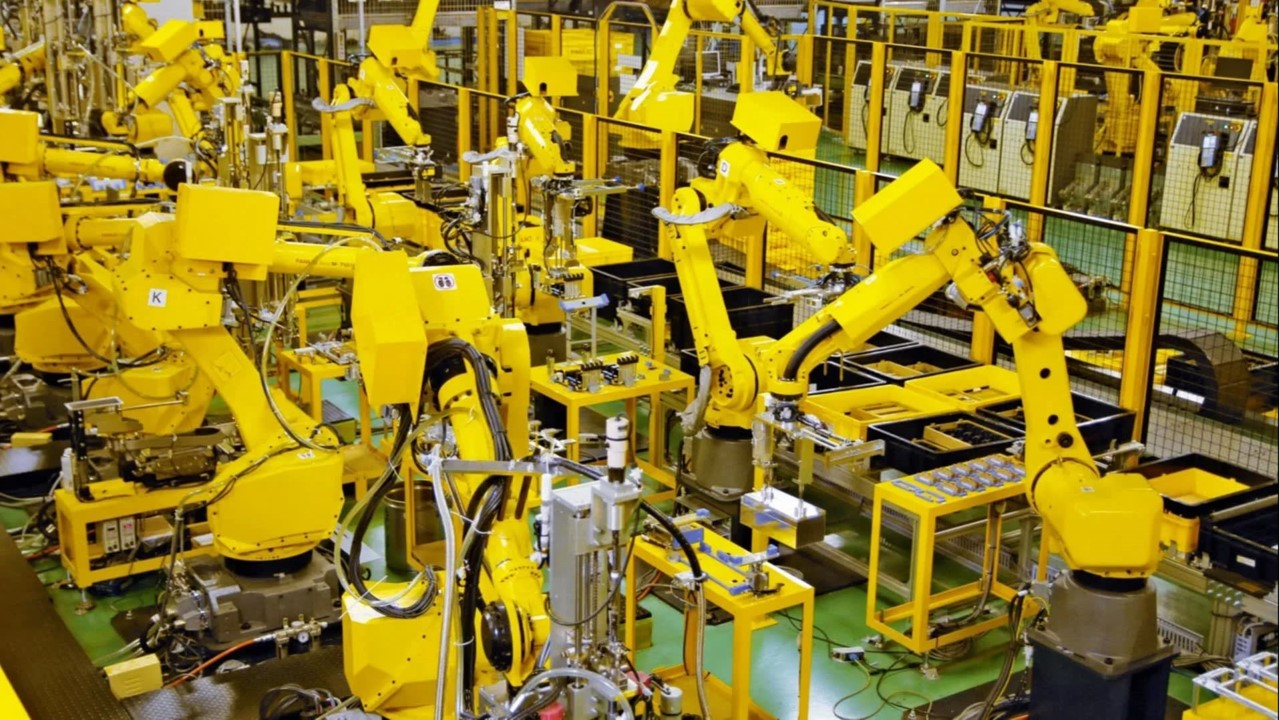
\includegraphics[width=\linewidth]{Picture2.jpg}
  \caption{Robot arms}
\endminipage

\end{figure}

But beware, this is not the whole answer!

\end{flushleft}
\end{frame}



\begin{frame}{Why Control?}
% \framesubtitle{Part 1}
\begin{flushleft}

The second most natural question to ask is - why do we need to study Control Theory? \emph{Why do Computer scientists need Control Theory?} 

\bigskip

\begin{exampleblock}{The easy answer is:}
it is very useful in case you will work in robotics, industrial automation, self-driving vehicles, drones, aerospace, etc.
\end{exampleblock}

\bigskip

\begin{alertblock}{But!}
this answer does not tell the main part of the story - what about people who are NOT going to work in the listed areas?
\end{alertblock}

\end{flushleft}
\end{frame}


\begin{frame}{Control as an applied problem}
\begin{flushleft}

We propose to view Control Theory as not only yet-another-subject. Instead we can try to see Control Theory course as \textbf{an application of your combined skills as a CS student}

\end{flushleft}
\end{frame}


\begin{frame}{Control as an applied problem}
\framesubtitle{Skills you will learn and practice}
\begin{flushleft}

In this course we provide you with learning and practical tasks that require:

\begin{itemize}
    \item Linear Algebra, Differential Equations, Computational methods
    \item Dynamical systems, Stability (concept build on top of Theory of Ordinary Differential Equations).
    % \item Linear dynamical systems (a deep look into one of the most useful and reach in scientific results areas of dynamical systems theory)
    
    \item Simulation of dynamical systems (closely related to computational methods in Differential Equations), as a programming problem.
    \item Development of experiments in Google Colab, using Python, mathematical libraries, solving concrete, real world-related math-oriented problems.
    
    \item Representation (parametrization) of equations as a tool in both mathematical analysis and simulation, software development and problem solving.
    
    \item ...and many other things.
\end{itemize}

\end{flushleft}
\end{frame}


\begin{frame}{...so, why Control?}
% \framesubtitle{Part 1}
\begin{flushleft}

Control Theory, as given here, is focused on:

\begin{enumerate}
    \item Giving you a challenge to simultaneously learn a new concepts, new general and subject-specific math, and new programming tools.
    \item Providing you with clear outcomes in terms of \emph{understanding} and ability to \emph{solve well-defined and meaningful real-world problems}.
    \item Being very useful for those who will proceed to work in robotics, automation, self-driving vehicles, drones, etc.
\end{enumerate}

See it as a test case for your abilities as a CS specialist.

\end{flushleft}
\end{frame}



\begin{frame}{Enough for the motivation}
% \framesubtitle{Part 1}
\begin{flushleft}


\begin{exampleblock}{Now that we know (kinda) why we do it:}

\hfill \break
Let's start with the content of the course!
\newline

\end{exampleblock}

\end{flushleft}
\end{frame}




\begin{frame}{Ordinary differential equations}
\framesubtitle{1st order}
\begin{flushleft}

Let us remember the normal form of first-order \emph{ordinary differential equations (ODEs):}

\begin{equation}
    \dot{\bo{x}} = \bo{f} (\bo{x}, t)
\end{equation}

where $\bo{x} = \bo{x}(t)$ is the solution of the equation and $t$ is a free variable.

\bigskip

\begin{definition}
We can call this equation (same as any other ODE) a \emph{dynamical system}, and $\bo{x}$ is called the \emph{state} of the dynamical system.  
\end{definition}

\begin{example}
\begin{equation}
    \dot{x} = -3 x^3 - 7 
\end{equation}
\end{example}

\end{flushleft}
\end{frame}






\begin{frame}{Ordinary differential equations}
\framesubtitle{n-th order}
\begin{flushleft}

The normal form of an \emph{n-th order} ordinary differential equation is:

\begin{equation}
    x^{(n)} = f (x^{(n-1)}, x^{(n-2)}, ..., \ddot{x}, \dot{x}, X, t)
\end{equation}

where $x = x(t)$ is the solution of the equation. Same as before, it is a \emph{dynamical system}, but this time the set $\{ x, \ \dot{x} \ ..., \ x^{(n-1)} \}$ is called the \emph{state} of the dynamical system.

\begin{example}
\begin{equation}
    \ddot{x} = cos(2\dot{x}) - 10 x + 7 
\end{equation}
\end{example}


\begin{example}
\begin{equation}
\begin{cases}
    \dddot{x}_1 = \dot{x}_1 + x_1 + x_2^2 - 4 \\
    \dddot{x}_2 = 10 x_1^3 + \ddot{x}_2
\end{cases}
\end{equation}
\end{example}

\end{flushleft}
\end{frame}




\begin{frame}{Linear differential equations}
\framesubtitle{1st order}
\begin{flushleft}

Linear ODEs of the first order have normal form:

\begin{equation}
    \dot{\bo{x}} = \bo{A} \bo{x} + \bo{b}
\end{equation}

\begin{example}
\begin{equation}
\begin{cases}
    \dot{x}_1 = -20 x_1 + 7 x_2 + 17 \\
    \dot{x}_2 = 10.5 x_1 - 3 x_2 - 5
\end{cases}
\end{equation}
\end{example}

\begin{example}
\begin{equation}
\begin{bmatrix}
\dot{x}_1 \\
\dot{x}_2 \\
\dot{x}_3
\end{bmatrix} 
= 
\begin{bmatrix}
-8   & 5   & 2  \\
 0.5 & -10 & -2 \\
 1   & -1 & -20
\end{bmatrix}
\begin{bmatrix}
x_1 \\
x_2 \\
x_3
\end{bmatrix} 
+
\begin{bmatrix}
4  \\
10 \\
-5
\end{bmatrix} 
\end{equation}
\end{example}

\end{flushleft}
\end{frame}




\begin{frame}{Linear differential equations}
\framesubtitle{n-th order}
\begin{flushleft}

A single linear ODE of the n-th order are often written in the form:

\begin{equation}
    a_n x^{(n)} + a_{(n-1)} x^{(n-1)} + 
    ... +
    a_2 \ddot{x} + a_1 \dot{x} + 
    a_0 x = b
\end{equation}

\begin{example}
\begin{equation}
12 \dddot{x} -
    3 \ddot{x} + 5.5 \dot{x} + 
    2 x = 10.5
\end{equation}
\end{example}

\begin{example}
\begin{equation}
    5 \ddot{x} - 2 \dot{x} + 
    10 x = 2
\end{equation}
\end{example}

\end{flushleft}
\end{frame}


\begin{frame}{Linear differential equations}
\framesubtitle{...are what we will study}
\begin{flushleft}

In this course we will focus entirely on linear dynamical systems. In particular, we will take a good use of the following two forms:

\begin{equation}
    a_n x^{(n)} + a_{(n-1)} x^{(n-1)} + 
    ... +
    a_2 \ddot{x} + a_1 \dot{x} + 
    a_0 x = b
\end{equation}

\begin{equation}
    \dot{\bo{x}} = \bo{A} \bo{x} + \bo{b}
\end{equation}

the last one is called \emph{state-space representation}.

\begin{exampleblock}{Good news:}

\hfill \break
Both of those can be used to express any linear system, hence we can change one into the other.
\newline

\end{exampleblock}

\end{flushleft}
\end{frame}




\begin{frame}{Changing n-th order ODE to a State-Space form}
% \framesubtitle{...are what we will study}
\begin{flushleft}

Consider eq. $\dddot{x} + a_2 \ddot{x} + a_1 \dot{x} + a_0 x = b$.

\bigskip

Make a substitution: $z_1 = x$, $z_2 = \dot{x}$, $z_3 = \ddot{x}$. Therefore:

\begin{equation}
    \begin{cases}
        \dot{z}_1 = \dot{x} = z_2 \\
        \dot{z}_2 = \ddot{x} = z_3 \\
        \dot{z}_3 =  -a_2 \ddot{x} - a_1 \dot{x} - a_0 x + b = 
        -a_2 z_3 - a_1 z_2 - a_0 z_1 + b
    \end{cases}
\end{equation}

Which can be directly put in the state-space form:

\begin{equation}
\begin{bmatrix}
\dot{z}_1 \\ \dot{z}_2 \\ \dot{z}_3
\end{bmatrix} 
=
\begin{bmatrix}
0 & 1 & 0 \\ 
0 & 0 & 1 \\
-a_0 & -a_1 & -a_2
\end{bmatrix} 
\begin{bmatrix}
z_1 \\ z_2 \\ z_3
\end{bmatrix} 
+ 
\begin{bmatrix}
0 \\ 0 \\ b
\end{bmatrix}
\end{equation}


\end{flushleft}
\end{frame}



\begin{frame}{State Space to ODE}
\centerline{An example of how linear algebra serves}
\centerline{to solve a seemingly difficult problem}
\bigskip
\centerline{(advanced, not going to be on the test)}
\end{frame}




\begin{frame}{State Space to ODE}
\framesubtitle{part 1}
\begin{flushleft}

Consider a system in state-space form:

\begin{equation}
\label{eq:SS}
\myvec{\dot x_1}{\dot x_2} = 
\ma{a_{11}}{a_{12}}{a_{21}}{a_{22}}
\myvec{x_1}{x_2} \ \ 
\Longleftrightarrow \ \ 
\dx{x} = \bo{A} \bo{x} 
\end{equation}

We want to find such equation 

\begin{equation}
\label{eq:ODE}
\ddot{y} + b_2 \dot{y} + b_1 y = 0
\end{equation}

that there exists a linear transformation of the initial conditions of \eqref{eq:SS} to the initial conditions of \eqref{eq:ODE}, such that the resulting solutions of the initial value problem for both \eqref{eq:SS} and \eqref{eq:ODE} can be transformed into one-another via another linear transformation.


\end{flushleft}
\end{frame}



\begin{frame}{State Space to ODE}
\framesubtitle{part 2}
\begin{flushleft}

We start by recognizing that differentiation is a linear operation, so $\dot{y}(t)$ is a linear transformation of \eqref{eq:ODE} of the solution $y(t)$. 

Next, we know that $y = \bo{w}^\top \bo{x}$ for some $\bo{w} = \myvecT{w_1}{w_2}$:

\begin{equation}
\dot y = \bo{w}^\top \bo{A} \bo{x}
\end{equation}

\begin{equation}
\dot y = \myvecT{(a_{11}w_1 + a_{21}w_2)}{(a_{12}w_1 + a_{22}w_2)}
\myvec{x_1}{x_2}    
\end{equation}

Analogous for $\ddot y$:

\begin{equation}
\ddot y = \bo{w}^\top \bo{A} \bo{A} \bo{x}
\end{equation}

\end{flushleft}
\end{frame}




\begin{frame}{State Space to ODE}
\framesubtitle{part 3}
\begin{flushleft}

Combining our results we find the linear transformation between the variables $x_1$, $x_2$ and $y$, $\dot y$:

\begin{equation}
\myvec{y}{\dot y} = 
\ma{w_1}{w_2}{(a_{11}w_1 + a_{21}w_2)}{(a_{12}w_1 + a_{22}w_2)}
\myvec{x_1}{x_2}    
\end{equation}

We can choose any $w_1$, $w_2$, as long as the resulting transformation matrix $\bo{T}$ is not degenerate:

\begin{equation}
\bo{T} = 
\ma{w_1}{w_2}{(a_{11}w_1 + a_{21}w_2)}{(a_{12}w_1 + a_{22}w_2)}
\end{equation}

\end{flushleft}
\end{frame}



\begin{frame}{State Space to ODE}
\framesubtitle{part 4}
\begin{flushleft}

Remember that:

\begin{equation}
    \ddot y = \bo{w}^\top \bo{A} \bo{A} \bo{x} \ \ 
    \Longleftrightarrow \ \ 
    \ddot{y} = -b_1 y -b_2 \dot{y}  = -\bo{b}^\top \myvec{y}{\dot y}
\end{equation}

Using the map we found previously, we obtain $\ddot y$ as a linear function of $y$, $\dot y$, with parameters $w_1$, $w_2$:

\begin{equation}
    \ddot y = \bo{w}^\top \bo{A} \bo{A} \bo{T}^+ \myvec{y}{\dot y}
\end{equation}

\begin{equation}
    \bo{b} = -\bo{w}^\top \bo{A} \bo{A} \bo{T}^+
\end{equation}

From this it is clear how the same can be generalized to higher dimensions.

\end{flushleft}
\end{frame}



\begin{frame}{State Space to ODE}
\framesubtitle{part 5}
\begin{flushleft}

\textcolor{blue}{\href{https://github.com/SergeiSa/Control-Theory-Slides-Spring-2022/blob/main/ColabNotebooks/StateSpace2ODE.ipynb}{Check out the code implementation.}}

\bigskip


\centerline{\textcolor{black}{\qrcode[height=2.1in]{https://github.com/SergeiSa/Control-Theory-Slides-Spring-2022/blob/main/ColabNotebooks/StateSpace2ODE.ipynb}}}


\end{flushleft}
\end{frame}




\begin{frame}{Read more}

\begin{itemize}
\item State Space Representations of Linear Physical Systems \href{https://lpsa.swarthmore.edu/Representations/SysRepSS.html}{lpsa.swarthmore.edu/Representations/SysRepSS.html}

\item Transformation: Differential Equation to State Space \href{https://lpsa.swarthmore.edu/Representations/SysRepTransformations/DE2SS.html}{lpsa.swarthmore.edu/.../DE2SS.html}
\end{itemize}

\end{frame}



\begin{frame}{Thank you!}
\centerline{Lecture slides are available via Moodle.}
\bigskip
\centerline{You can help improve these slides at:}
\centerline{\href{https://github.com/SergeiSa/Control-Theory-Slides-Spring-2021}{github.com/SergeiSa/Control-Theory-Slides-Spring-2021}}
\bigskip
\centerline{Check Moodle for additional links, videos, textbook suggestions.}
\end{frame}

\end{document}
